% !TeX root = repressed-anger.tex

\section{Emotion Detection}
\label{sec:emotion_detection}

Emotion detection has been always a important field of study in neuroscience and psychology. Several experiments have been conducted to recognize emotions from face expressions, voice and body gestures, such in \cite{bassili1979emotion}; \cite{banziger2009emotion} and \cite{gunes2007bi}. However, these features are not always available and thus, the detection of emotion from text has gain relevance during the last decade.

Emotion detection from text documents is closely related to \acrshort{sa}. As explained in \ref{subsubsection:sentiment_classification}, sentiment classification task consists in determine the polarity of a given text into two or more classes. Emotion detection also fits this description, since this field of study is conducted by classifying a given document into predefined emotion labels. The definition of these labels are based on previously presented emotion models, which consist on application psychological and neuroscientific theories to represent emotions. One of the first model defined was proposed by Paul Ekman, on 1972, composed by six basic emotions, \textit{``happiness, sadness, fear, anger, surprise and disgust''}, and has been used in multiple face recognition systems and is the base emotion detection from text \cite{StevenEmotion2011Classification} as its definition has resulted to be the most semantically diverse \cite{bann2013conceptualisation}.

\begin{figure}[!htp]
  \center
  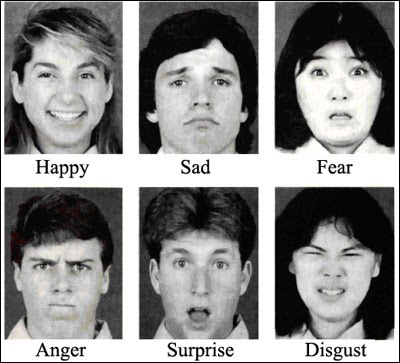
\includegraphics[width=0.5\textwidth]{figures/emotions_ekman}
  \caption{Ekamn's basic emotions, image extracted from Expressions, Emotions and Emblems, Google Sites.}
  \label{fig:ekman_basic_emotions}
\end{figure}

Since then, more interpretations have been made regarding the representation of the emotions as shown in \cite{cambria2012hourglass}. Ekman himself added his list 11 new emotions stating that not all of them could be represented by facial expressions. In 1980 Robert Plutchik created another bi-dimensional model (see figure \ref{fig:plutchik-wheeel}), known as wheel of emotions, that defined eight basic bipolar emotions with different levels of intensification and could be combined among them. \acrfull{occ} designed in 1988 a model in which emotions were driven by an agent, based on the premise that \textit{``emotions are not themselves linguistic things, but the most readily available non phenomenal access we have to them is through language''} \cite{binali2010computational}. The model included 22 emotion categories that aimed to \textit{``model humans in general''} \cite{binali2010computational}. \acrshort{occ} enables the study of emotions as classes that share the same feeling, instead of specific words, proving that this \textit{``is a theory of emotions and not a theory of the language of emotions''} \cite{binali2010computational}. For more information, authors of \cite{binali2012emotion} analyze the state of art of the emotion models and the techniques used to generate them.

\begin{figure}[!htp]
  \center
  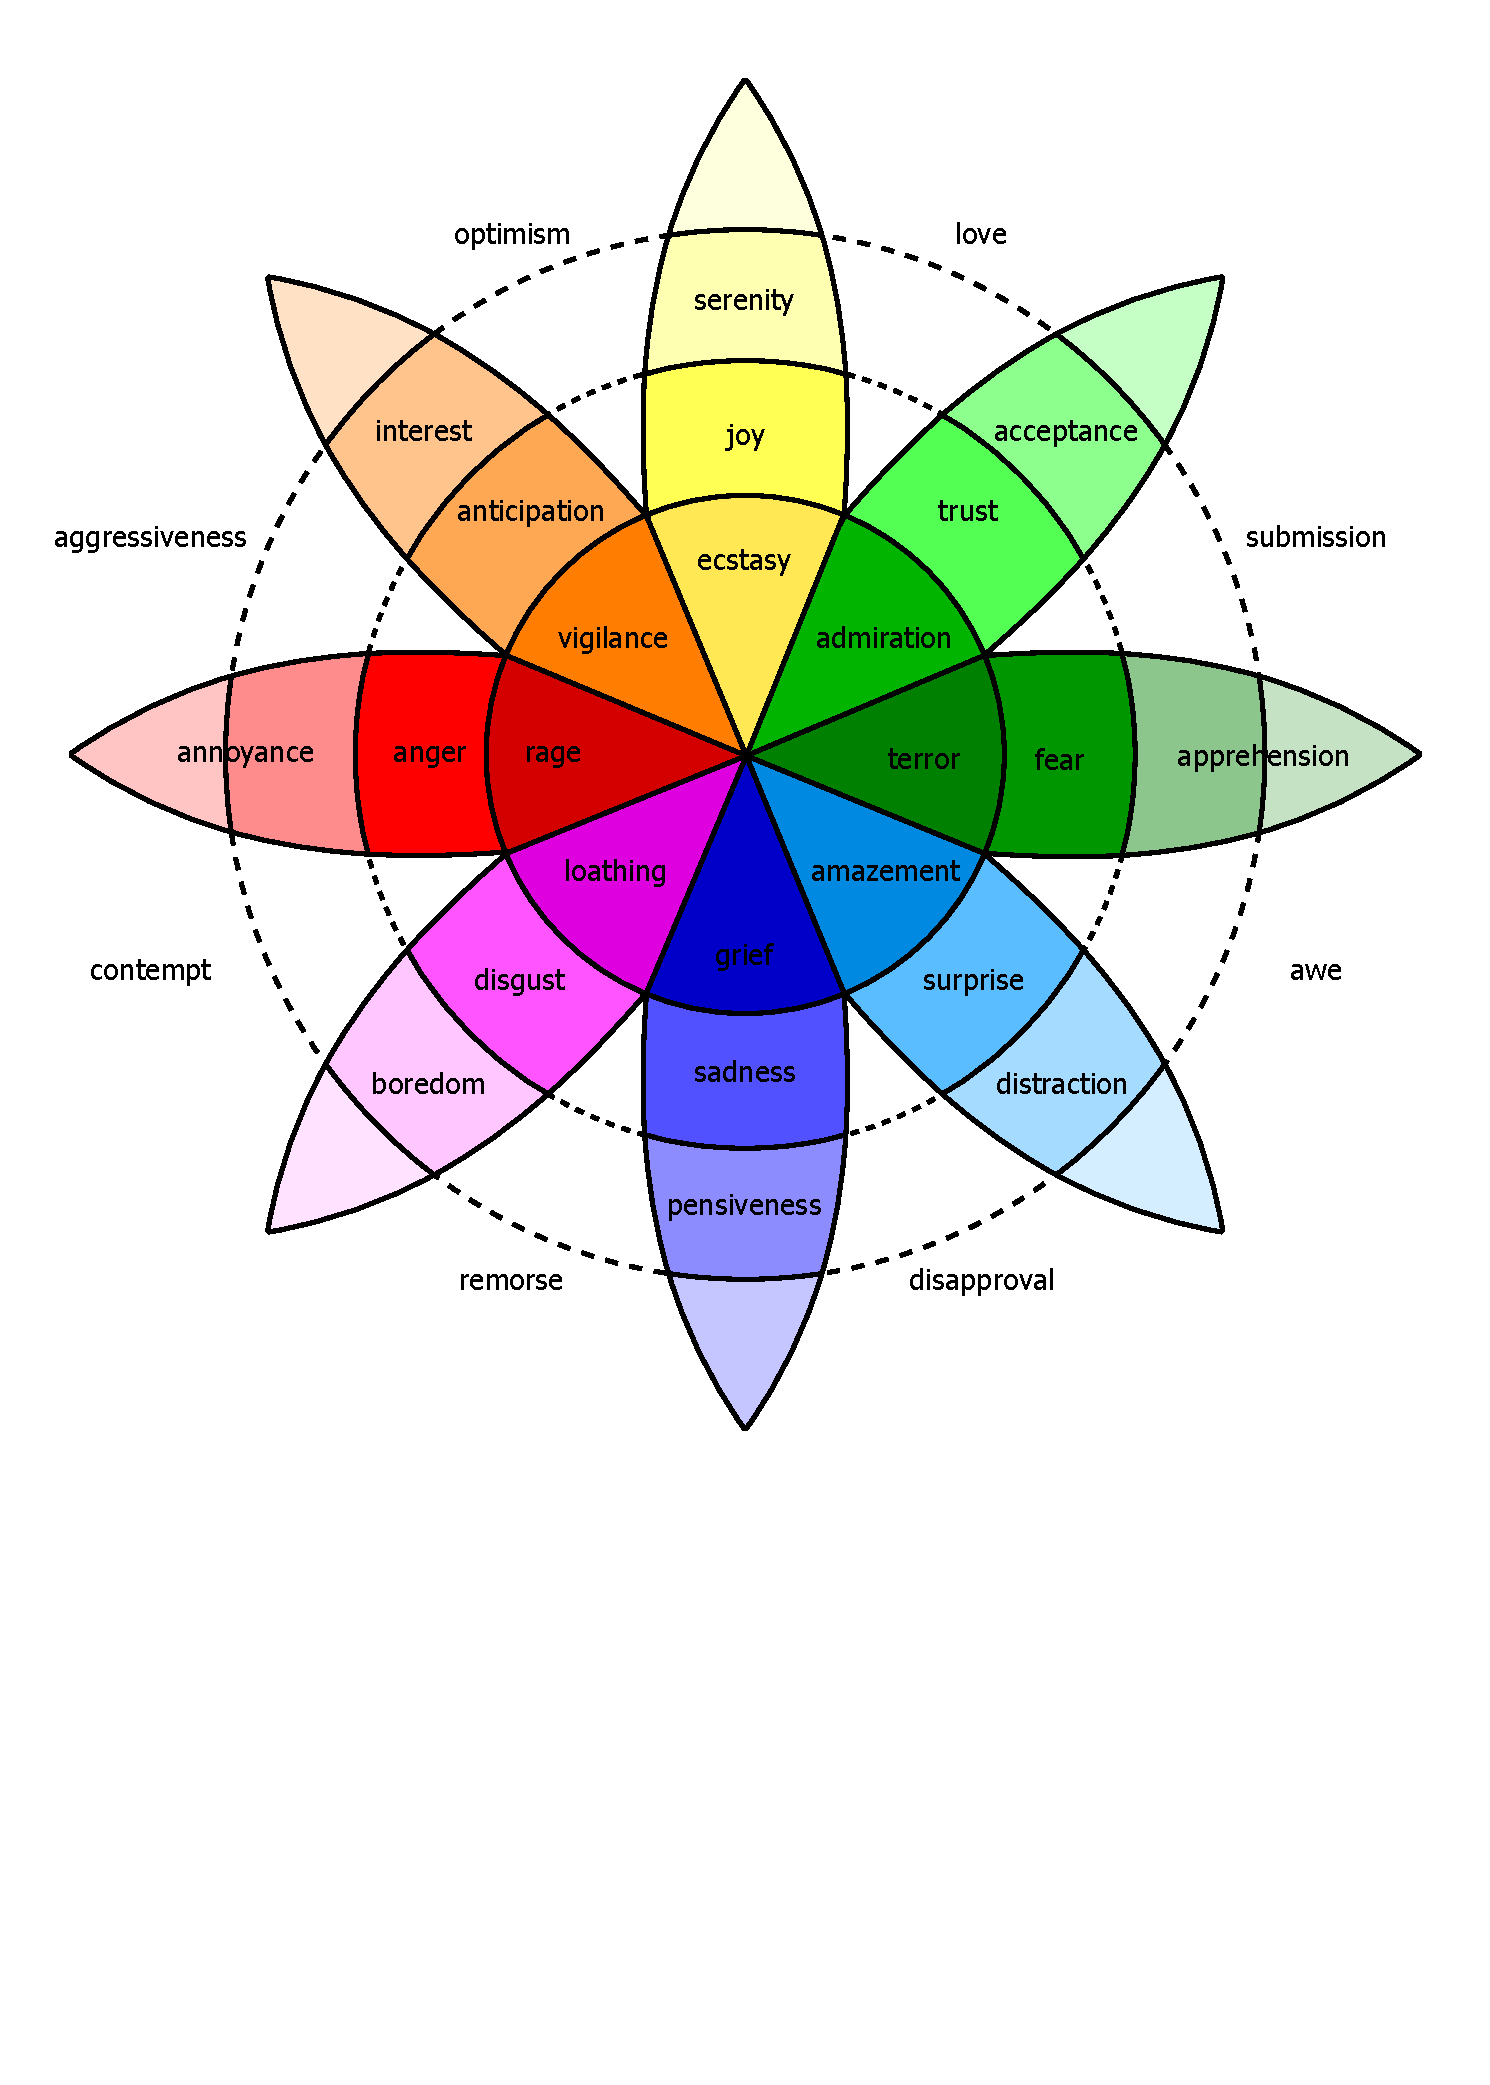
\includegraphics[width=0.6\textwidth]{figures/plutchik-wheel}
  \caption{Plutchik's emotion wheel, image extracted from Wikipedia's public domain.}
  \label{fig:plutchik-wheeel}
\end{figure}

Emotion classification tasks shares the same principles as \acrshort{sa}, and thus, the techniques used are mainly \acrshort{ml}, lexicon-based and hybrid approaches previously explained in section \ref{subsec:sentiment_analysis_techniques}.